\scanpage{2}
$V$ : \uline{\unsure{W.d.|V.d.|a.v.d.} noethérien}, complet
\[
\operatorname{Spec}(V)\qquad k\ \text{\unsure{corps résid.|corps résiduel}}\qquad K\ \text{\unsure{corps fractions|corps des fractions}}
\]
\unsure{Groupe galoisien|Gpe galoisien|Théorie galoisienne} $(K)$

a) $\operatorname{car}(k)=0$\qquad \uuline{$k$ alg clos}.
\figure{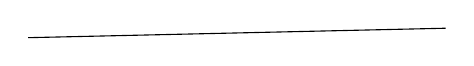
\begin{tikzpicture}\draw (0,0)--(5.3,.12);\end{tikzpicture}}
\unsure{Les|Ces} extens \unsure{de|a} $K$ sont \unsure{abél.} \unsure{cyclique|cycliques} donc \unsure{Kummerienne|Kummeriennes}.
\[
K^*/K^{*n}\simeq\mathbf Z/n\mathbf Z\qquad\text{(par la valuation)}
\]
Soit $\overline K$ clôture \unsure{de|a.} $K$.
\diagram{\begin{tikzcd}[ampersand replacement=\&,column sep=small,row sep=small]
\Gamma(\overline K,K) \arrow[r,phantom,"\overset{\text{not}}{=}"] \& T_\infty(k) \arrow[r,phantom,"="] \& \displaystyle\varprojlim_n\underbrace{\mu_n(k)} \arrow[d,phantom,"\wr"] \& (\simeq\widehat{\mathbf Z})\\
\&\&\mathbf Z/n\mathbf Z
\end{tikzcd}}
\figure{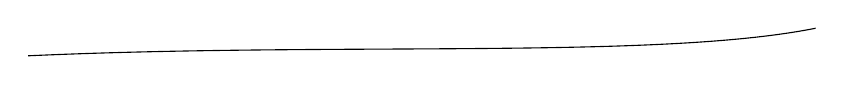
\begin{tikzpicture}\draw (0,0)..controls (4,.18) and (8,-.05)..(10,.35);\end{tikzpicture}}
si $k$ car $\unsure{\ne0|p>0}$ $V$ pas néces. complet,
\[
\underset{\text{prem à }p}{\pi_1(K)}\longrightarrow\varprojlim_{n\text{ prem à }p}\mu_n(\unsure{k|K})
\]
\mspage{1}
